\documentclass[10pt,a4paper,final]{article}
\usepackage[utf8]{inputenc}
\usepackage[portuguese]{babel}
\usepackage[T1]{fontenc}
\usepackage[margin=1in]{geometry}
\usepackage{amsmath}
\usepackage{amsfonts}
\usepackage[table]{xcolor}
\usepackage{graphicx}
\usepackage{multirow}
\usepackage{setspace}
\usepackage{amssymb}
\usepackage{lscape}
\usepackage{plano}
%\usepackage[alf]{abntex2cite}
\usepackage{natbib}
\usepackage{hyperref}
\usepackage{csquotes}

\programa{Engenharia Elétrica}
\area{Engenharia de Computação}
\aluno{Jefferson Carlos de Mendonça}
\orientador{Prof. Dr. Edson Satoshi Gomi}
\curso{Mestrado}
\dataIngresso{14/09/2016}
\titulo{Algoritmo para categorização das Perguntas do \textit{Site Stack Overflow}}
\resumo{Transformações no cenário tecnológico provocam mudanças constantes e exigem atualização contínua. Para manter-se atualizado, profissionais da área de computação recorrem à diversas fontes de informação, dentre elas destaca-se o site \textit{Stack Overflow}[1], maior comunidade de perguntas e respostas, onde os usuários podem aprender, trocar experiências e compartilhar conhecimento.
O objeto de pesquisa deste trabalho é propor um algoritmo que consiga categorizar as perguntas deste \textit{website}. Uma vez que os questionamentos estejam devidamente indexados e organizados em tópicos, será possível detectar as dúvidas mais frequêntes reportadas pelos usuários, permitindo que um assunto seja encontrado com maior facilidade, além de permitir que as entidades dententoras das tecnologias envolvidas, use os resultados obtidos para criar manuais e cursos que potencialize o ententimento da comunidade de interesse.}

\palavrachave{recuperação de informação}
\palavrachave{mineração de textos}
\palavrachave{classificação de textos}
\palavrachave{categorização automática de textos}
\palavrachave{extração de palavras chave}
\palavrachave{indexação de documentos}
\palavrachave{stack overflow}


\begin{document}

    \folhaDeRosto

    \plano
    
    \section{Introdução}
    
A evolução na área computacional se desenvolve em ritmo acelerado, algoritmos, técnicas para programação distribuída, testes automatizados, bancos de dados e outros assuntos possuem algo em comum, eles mudam com frequência. Com as \emph{linguagens de programação} não é diferente, suas API's são aprimoradas constantemente e muitas vezes elas incorporam novos paradigmas. Para acompanhar estas mudanças, profissionais da área de computação necessitam qualificação, que pode ser obtida através de cursos presenciais, a distância, livros, revistas, artigos e claro \textit{websites}.
\newline
\newline
 \cite{Manning2009} afirmam que a \textit{web} tornou-se a principal fonte por busca de informação e o relatório elaborado por \cite{Fallows} conclui que \enquote{ 92\% dos internautas dizem que a internet é um bom lugar para obter informações diariamente }.
Dentre estas fontes, merece destaque o fórum \textit{Stack Overflow} (SO), maior comunidade \textit{online} de perguntas e respostas onde os usuários podem aprender, trocar experiências e compartilhar conhecimento.
    
    \subsection{Contextualização do Problema}
O número de questões em sites de perguntas e respostas cresce diariamente, faz-se necessário categorizar os assuntos discutidos em tópicos, para uma busca mais eficiente e rápida. \cite{Manning2009} comparam este problema ao da procura de um livro em uma biblioteca, com certeza nossa busca será mais rápida e assertiva se os livros estiverem separados em prateleiras por assunto ou tópico. \cite{Yasotha2016} adicionam que a categorização manual de textos pode ser feita somente por especialistas e essa tarefa requer muito tempo. Como consequência é de grande importância a categorização e classificação de documentos de forma automática, ajudando os usuários a encontrarem informações relevantes para as suas necessidades.

    \subsection{Objetivos}
A proposta deste projeto de pequisa, é desenvolver um algoritmo que categorize e classifique os assuntos discutidos no SO, que faça uso apenas do texto disponível nas perguntas e respostas, sem que haja a necessidade de recorrer ao uso de tags.

    \subsection{Justificativas}

O método muito bem detalhado por \cite{Arash2016} categoriza os dados do SO. Em seu projeto os autores classificaram os assuntos utilizando as tags da própria pergunta. No SO o próprio usuário, elege qual é a tag da referida pergunta publicada. Apesar do grande avanço nesse campo de pesquisa, o uso de tags limita a expansão da solução para outros fórums que não possuem este recurso, como por exemplo os \textit{sites} Quora[2] e Code Ranch[3].

   \subsection{Organização do texto}

Para melhor definir qual o posicionamento do presente projeto, no capítulo seguinte será detalhado em maior profundidade os projetos que abordaram a categorização de documentos, inclusive àqueles que também fizeram uso do site \textit{Stack Overflow} como base de dados. Então a proposta será detalhada quantos aos procedimentos para a indexação das perguntas e respostas, desde a seleção do conteúdo original, armazenamento em banco de dados e extração, por fim serão exibidos os resultados esperados. Segundo \cite{Kaleta2014} o termo indexação pode ser entendido como um dicionário de palavras-chave que representam o conteúdo de um texto.	

 \section{Revisão da Literatura}
   Revisão da literatura (item pendente).


 \section{Detalhamento da Proposta}

Dados de 2008 apontam que o SO recebe cerca de 7.000 questões por dia, \cite{Krippendorff2012} sublinha que a mineração de texto vem sendo adotada como uma alternativa à situações em que a análise manual de grande quantidade dados se torna inviável. Análogo a metodologia proposta por \cite{Arash2016} a figura 1 exemplifica o processamento da informação desde sua obtenção até a produção dos resultados finais.
\newline
\newline
A primeira etapa é composta pela \textbf{coleta da informação}, o SO faz parte da rede de \textit{websites} StackExchange[4] que adota uma política de acesso livre à informação, ou seja, as postagens - perguntas e respostas, os usuários e os comentários são Periódicamente disponibilizados de forma gratuita[5] para download e análise.
\newline
\newline
Na etapa de \textbf{extração da informação} será desenvolvido um algoritmo para extrair os assuntos principais \cite{Turney:2000:LAK:593957.593993} das dúvidas postadas no \textit{site}, assim como na proposta anterior também será utilizado o Wikipédia Miner \cite{Milne2012} como base de conhecimento sobre o vocabulário (palavras-chave) encontrado, de forma complementar também serão armazados a quantidade de vizualizações, a pontuação atribuída e o número de respostas da referida pergunta.
\newline
\newline
Por fim, na fase de \textbf{mineração do texto} será criado um \textit{ranking} \cite{mihalcea-tarau:2004:EMNLP} dos tópicos relevantes questionados com mais frequência, será utlizado o Gephi \cite{ICWSM09154} software \textit{open source} para exibir o grafo das categorias e suas interconexões.

\begin{figure}[!htb]
\centering
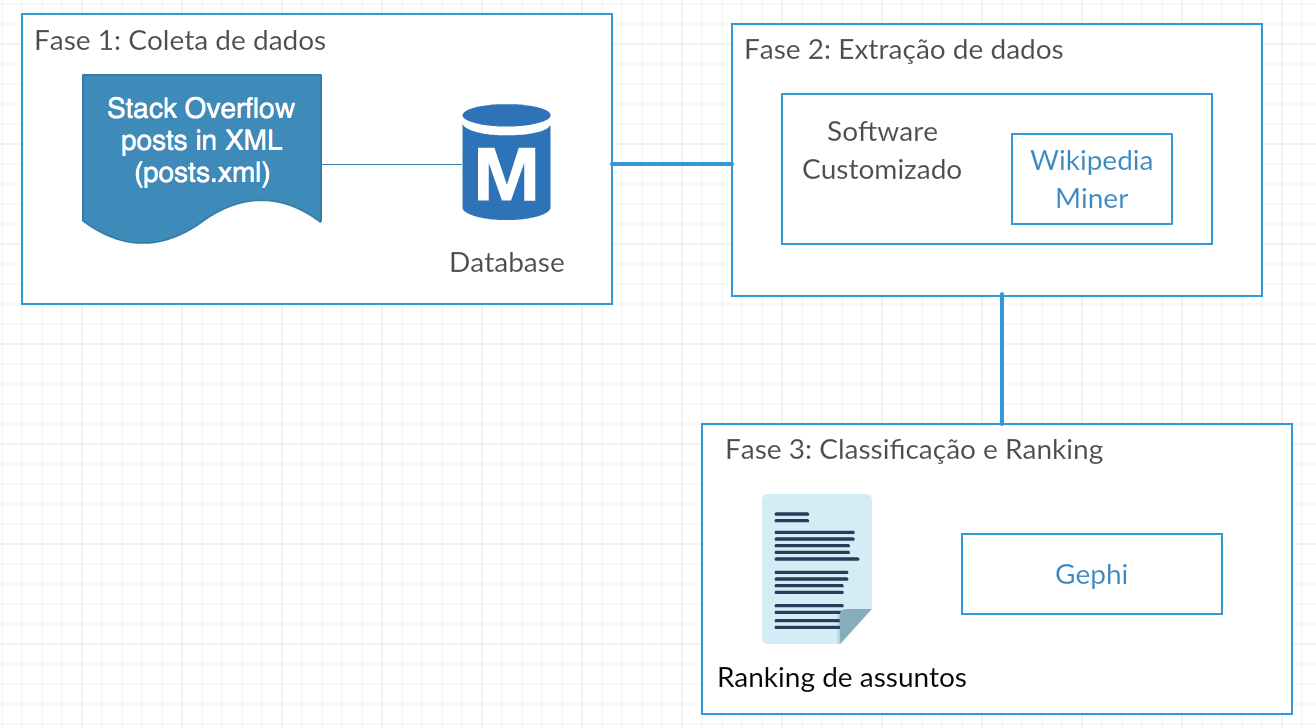
\includegraphics[height=8cm]{Figures/figura_1_metodologia}
\label{fig:figura_1_metodologia}   
\caption{Visão geral para categoriazação de perguntas e resposta do Stack Overflow.}
\end{figure}

  
    \section{Plano de Trabalho}

    \subsection{Resultados Desejados e Validação}
    
A análise será feita sobre os mesmo dados da pesquisa realizada por \cite{Arash2016}, os resultados obtidos anteriormente serão a base para a medição da acurácia da nova proposta e então será possível aplicar o modelo desenvolvido sem a utilização de tags pré-definidas, possibilitando a construção de catálogos para outros sites de perguntas e respostas.
 
    \subsection{Atividades e Cronograma}
    
Atividades:
    \begin{itemize}
    \item Disciplinas
	\item[] \quad Machine Learning
    \item[] \quad Metodologia Científica
    \item[] \quad Ciência de Dados
    \item[] \quad Inteligência Artificial
    \item[] \quad Fundamentos Engenharia de Computação
    \item Revisão Literária
    \item Plano de Pesquisa
    \item Artigo Científico
    \item Projeto de Pesquisa
    \item[] \quad Fase 1: Coleta de dados
    \item[] \quad Fase 2: Extração de dados
    \item[] \quad Fase 3: Classficação e \textit{Ranking}
    \item Qualificação
    \item Defesa
    \end{itemize}

% ----------------------------------------------------------
% Cronograma
% ----------------------------------------------------------

\begin{figure}[!htb]
\centering
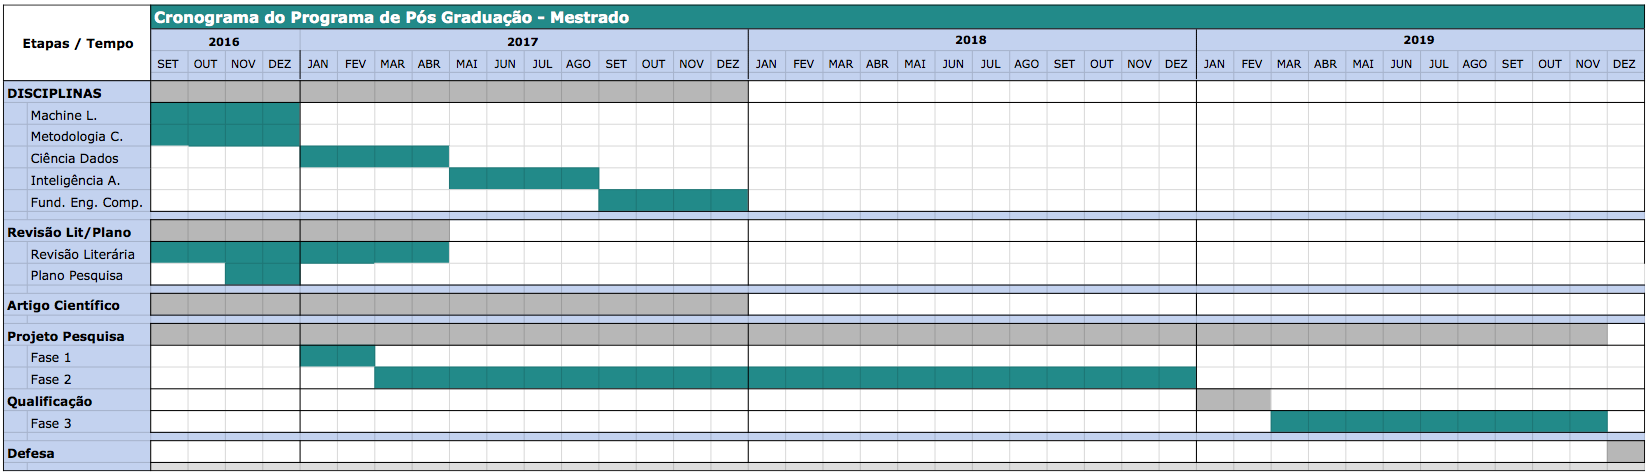
\includegraphics[height=4.8cm]{Figures/cronograma_projeto_project_timeline_retrato}\label{fig:cronograma_projeto_project_timeline_retrato}   
\caption{Cronograma.}
\end{figure}


% ----------------------------------------------------------
% Notas para links externos
% ----------------------------------------------------------

%%\chapter{Notes}
\textbf{\newline Notas}
\newline
\newline
1. http://stackoverflow.com/tour \newline
2. http://www.quora.com \newline
3. http://coderanch.com \newline
4. http://stackexchange.com \newline
5. https://archive.org/download/stackexchange

% ----------------------------------------------------------
% Referências bibliográficas
% ----------------------------------------------------------
\nocite{Joorabchi2015}
\nocite{Manning2009}
\nocite{Mihalcea2007}
\nocite{Mihalcea2001}
\nocite{Mihalcea2004}
\nocite{Milne}
\nocite{Miotto2013}
\nocite{Posch2014}
\nocite{Roul2015}
\nocite{Udell2005}
\bibliographystyle{apalike}
\bibliography{Refs}{}  


    

\end{document}
    